\documentclass{curs}

% Comment out lines below in case of no code to be included.
%\usepackage{code/highlight}
\usepackage{color}
\usepackage{graphicx}
%\usepackage{alltt}


\title[Session 02]{Session 02}
\subtitle{Authentication}
\author{Security of Information Systems (SIS)}
\date{October 4, 2019}

\begin{document}

\frame{\titlepage}


\begin{frame}{Access Control Terms}
  \begin{itemize}
    \item authentication
    \item authorization
    \item access control
  \end{itemize}
\end{frame}

\section{Authentication}

\begin{frame}{Model}
  \begin{itemize}
    \item actor / subject / agent
    \item credentials database (role, permissions, access control list)
    \item resource / object
    \item reference monitor
  \end{itemize}
\end{frame}

\begin{frame}{Credentials}
  \begin{itemize}
    \item who you are
    \item what you have
    \item what you know
  \end{itemize}
\end{frame}

\begin{frame}{Credential Types}
  \begin{itemize}
    \item biometric
    \item hardware tokens
    \item software tokens
    \item secret (password)
  \end{itemize}
\end{frame}


\section{Credentials}

\begin{frame}{Biometrics}
  \begin{itemize}
    \item fingerprint
    \item face
    \item iris
    \item voice
    \item keystroke dynamics
  \end{itemize}
\end{frame}

\begin{frame}{Hardware Tokens}
  \begin{itemize}
      \item access card
      \item hardware keys
      \item one-time password (OTP)
    \end{itemize}
\end{frame}

\begin{frame}{Software Tokens}
  \begin{itemize}
    \item certificate
    \item kerberos ticket
    \item cookie
  \end{itemize}
\end{frame}


\section {Password-based Access}

\begin{frame}{Passwords}
  \begin{itemize}
    \item string of printable characters (ASCII)
    \item protect access
    \item stored in a password database and requested at each
      login/authentication
    \item most common method of authentication
  \end{itemize}
\end{frame}

\begin{frame}{Password Cracking Context (1)}
  \begin{figure}
    \centering
    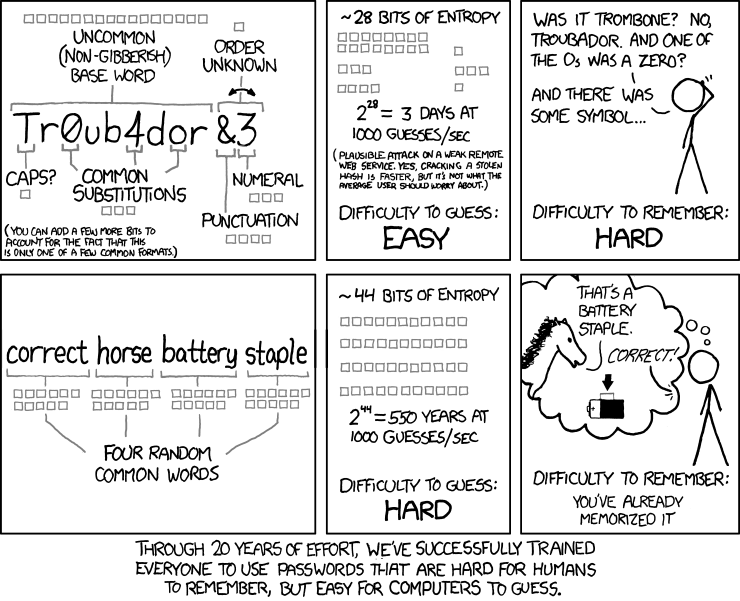
\includegraphics[width=0.8\textwidth]{img/password-strength.png} \\
    \tiny{\url{http://xkcd.com/936/}}
  \end{figure}
\end{frame}

\begin{frame}{Password Cracking Context (2)}
  \begin{figure}
    \centering
    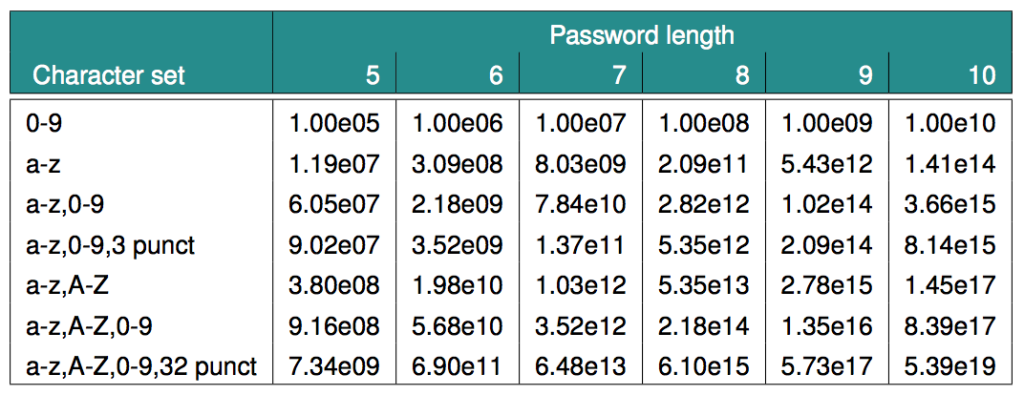
\includegraphics[width=0.8\textwidth]{img/password-complexity.png} \\
    \tiny{\url{http://hitachi-id.com/password-manager/docs/password-management-best-practices.pdf}}
  \end{figure}
\end{frame}

\begin{frame}{Passwords vs. Passphrases}
  \begin{itemize}
    \item a password is a word and a passphrase is a set of words
    \item passphrases usually has spaces
    \item passphrases are recommended due to their increased length and being easier to remember
  \end{itemize}
\end{frame}

\begin{frame}{Attacker}
  \begin{itemize}
    \item online attack
      \begin{itemize}
        \item ``live'' attack
        \item run client/application, feed passwords and try to match
      \end{itemize}
    \item offline attack
  \end{itemize}
\end{frame}

\begin{frame}{Scenario 1: Plaintext}
  \begin{itemize}
    \item attacker
      \begin{itemize}
        \item gain access to database
        \item profit!
      \end{itemize}
    \item defender
      \begin{itemize}
        \item database access control
        \item one-way function
      \end{itemize}
  \end{itemize}
\end{frame}


\section{Securing Password-based Access}

\begin{frame}{Cryptographic Hash Functions}
  \begin{itemize}
    \item deterministic
    \item uniformity
    \item infeasible to reverse
    \item highly dynamic
    \item usually very fast
  \end{itemize}
\end{frame}

\begin{frame}{Hash Security Properties}
  \begin{itemize}
    \item pre-image resistance
    \item second pre-image resistance
    \item collision resistance
  \end{itemize}
\end{frame}

\begin{frame}{Hash Algorithms}
  \begin{itemize}
    \item \color{red}SHA1
    \item \color{red}MD2, MD4, MD5
    \item \color{lime}SHA2
    \item \color{green}bcrypt
    \item \color{green}SHA3
  \end{itemize}
\end{frame}

\begin{frame}{Scenario 2: Hashed Password}
  \begin{itemize}
    \item attacker
      \begin{itemize}
        \item rainbow tables
        \item profit!
      \end{itemize}
    \item defender
      \begin{itemize}
        \item salt
      \end{itemize}
  \end{itemize}
\end{frame}

\begin{frame}{Rainbow Tables}
  \begin{itemize}
    \item database of hashes
    \item space vs time
  \end{itemize}
\end{frame}

\begin{frame}{Rainbow Tables (2)}
  \begin{figure}
    \centering
    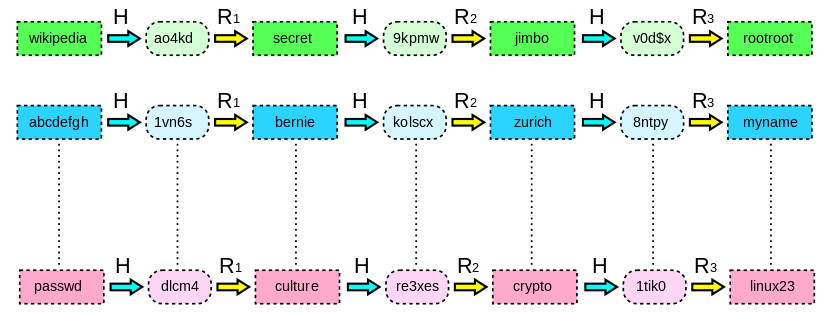
\includegraphics[width=0.9\textwidth]{img/rainbow-table.png} \\
    \tiny{\url{http://en.wikipedia.org/wiki/Rainbow_table}}
  \end{figure}
\end{frame}

\begin{frame}{Salt}
  \begin{itemize}
    \item Additional input
    \item Concatenated with the password
    \item One per password
  \end{itemize}
\end{frame}

\begin{frame}{Scenario 3: Salted hashes}
  \begin{itemize}
    \item attacker
      \begin{itemize}
        \item dictionary / hybrid attack
        \item brute-force attack
        \item side-channel attacks
        \item profit ?!?
      \end{itemize}
    \item defender \begin{itemize}
      \item policies
      \item defensive programming
    \end{itemize}
  \end{itemize}
\end{frame}

\begin{frame}{Dictionary Attacks}
  \begin{itemize}
    \item use a dictionary/word list
    \item go through word list, compute hash and compare to password hash
    \item simple form of attack
    \item relies on people using simple passwords
  \end{itemize}
\end{frame}

\begin{frame}{Password Dictionaries / Word Lists}
  \begin{itemize}
    \item \url{http://wiki.skullsecurity.org/Passwords}
    \item \url{https://crackstation.net/buy-crackstation-wordlist-password-cracking-dictionary.htm}
    \item \url{http://security.stackexchange.com/questions/9567/modern-high-quality-password-dictionary}
  \end{itemize}
\end{frame}

\begin{frame}{Hybrid Attack}
  \begin{itemize}
    \item use a dictionary
    \item apply mutations for each word
      \begin{itemize}
       \item combine dictionary words
        \item change i to 1, s to 5, e to 3
        \item change cases
        \item add 123 at the end of the word
        \item add ! at the end of the word
      \end{itemize}
    \item hash and check with password hash
  \end{itemize}
\end{frame}

\begin{frame}{Policy}
  \begin{itemize}
    \item complexity
      \begin{itemize}
        \item password length
        \item charset
      \end{itemize}
    \item password expiration
    \item password reuse
  \end{itemize}
\end{frame}

\begin{frame}{Policy Issues}
  \begin{itemize}
    \item password security paradox
      \begin{itemize}
        \item easy to remember
        \item hard to guess
      \end{itemize}
    \item user behavior
    \item solution: password managers
  \end{itemize}
\end{frame}

\begin{frame}{Side-Channel Attacks}
  \begin{itemize}
    \item timing information
    \item performance / power consumption 
    \item electromagnetic leak
    \item acoustic information
    \item social engineering
    \item rubber-hose technique
  \end{itemize}
\end{frame}

\begin{frame}{Rubber-hose technique}
  \begin{figure}
    \centering
    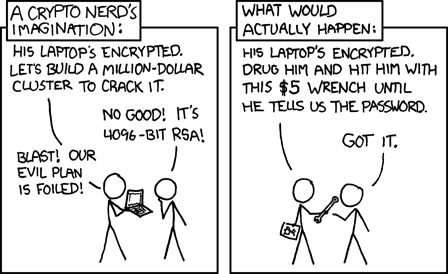
\includegraphics[width=0.8\textwidth]{img/security-wrench.png} \\
    \tiny{\url{http://xkcd.com/538/}}
  \end{figure}
\end{frame}


\section{Summary}

\begin{frame}{Recommendations}
  \begin{itemize}
    \item do not use unsafe hashing algorithms!!!
    \item passphrase $>$ complex password
    \item use / allow password managers
    \item use 2FA / 3FA
    \item secure side channels
  \end{itemize}
\end{frame}

\begin{frame}{Common tools}
  \begin{itemize}
    \item \href{http://www.openwall.com/john/}{John The Ripper}
    \item \href{http://project-rainbowcrack.com/}{RainbowCrack}
    \item \href{https://hashcat.net/hashcat/}{HashCat}
  \end{itemize}
\end{frame}

\begin{frame}{Keywords}
  \begin{columns}
    \begin{column}{0.5\textwidth}
      \begin{itemize}
        \item credentials
        \item password
        \item passphrase
        \item hash functions
        \item rainbow tables
        \item salt
        \item dictionary attack
        \item side-channel attack
        \item policies
      \end{itemize}
    \end{column}
    \begin{column}{0.5\textwidth}
      \begin{itemize}
        \item social engineering
        \item shoulder surfing
        \item one-time password
        \item password complexity
        \item password manager
        \item 2/3 factor authentication
        \item SHA256, SHA512
        \item sHA3
        \item rubber-hose technique
      \end{itemize}
    \end{column}
  \end{columns}
\end{frame}

\begin{frame}{Nice to read}
  \begin{itemize}
    \item \href{http://books.expect-us.net/dl/Password_Cracking_Techniques.pdf}{Password Cracking Techniques}
    \item \href{https://arstechnica.com/information-technology/2017/05/breaking-the-iris-scanner-locking-samsungs-galaxy-s8-is-laughably-easy/}{Breaking the iris scanner locking Samsung’s Galaxy S8 is laughably easy}
    \item \href{https://arstechnica.com/gadgets/2017/03/video-shows-galaxy-s8-face-recognition-can-be-defeated-with-a-picture/}{Galaxy S8 face recognition already defeated with a simple picture}
    \item \href{https://arstechnica.com/information-technology/2013/09/touchid-hack-was-no-challenge-at-all-hacker-tells-ars/}{Bypassing TouchID was “no challenge at all,” hacker tells Ars}
    \item \href{https://paul.reviews/behavioral-profiling-the-password-you-cant-change/}{Behavioral Profiling: The password you can't change.}
  \end{itemize}
\end{frame}
\end{document}
